\chapter{再現実験を含めた事象選別と結果(担当:礒部)}\label{result}

超微細構造の測定にはポジトロニウムの寿命を求める必要がある.
そのため,超微細構造の測定に先立ち昨年度の再現実験を行い真空中でのオルソポジトロニウムの寿命測定を試みた.

\section{再現実験の実験装置}
昨年度の測定~\cite{卒業論文2015}を参考にし,同様のセットアップで行った.
図\ref{fig:setting2015}と図\ref{fig:pmt_setting2015}にそれぞれ装置の全体図とシンチレータA,B,Cの配置の写真を,図\ref{fig:setting_dtl2015}に装置の概要図を示す.
\begin{figure}[htbp]
	\begin{tabular}{cc}
		%1枚目
		\begin{minipage}{0.5\hsize}
			\centering
				\includegraphics[width=80mm]{img/isb/setting_overview.JPG}
				\caption{装置の全体写真}
				\label{fig:setting2015}
		\end{minipage}
		%2枚目
		\begin{minipage}{0.5\hsize}
			\centering
			\includegraphics[width=80mm]{img/isb/pmt_setting.JPG}
				\caption{シンチレータA,B,Cの配置}
				\label{fig:pmt_setting2015}
		\end{minipage}
	\end{tabular}
\end{figure}

\begin{figure}[H]
	\centering
		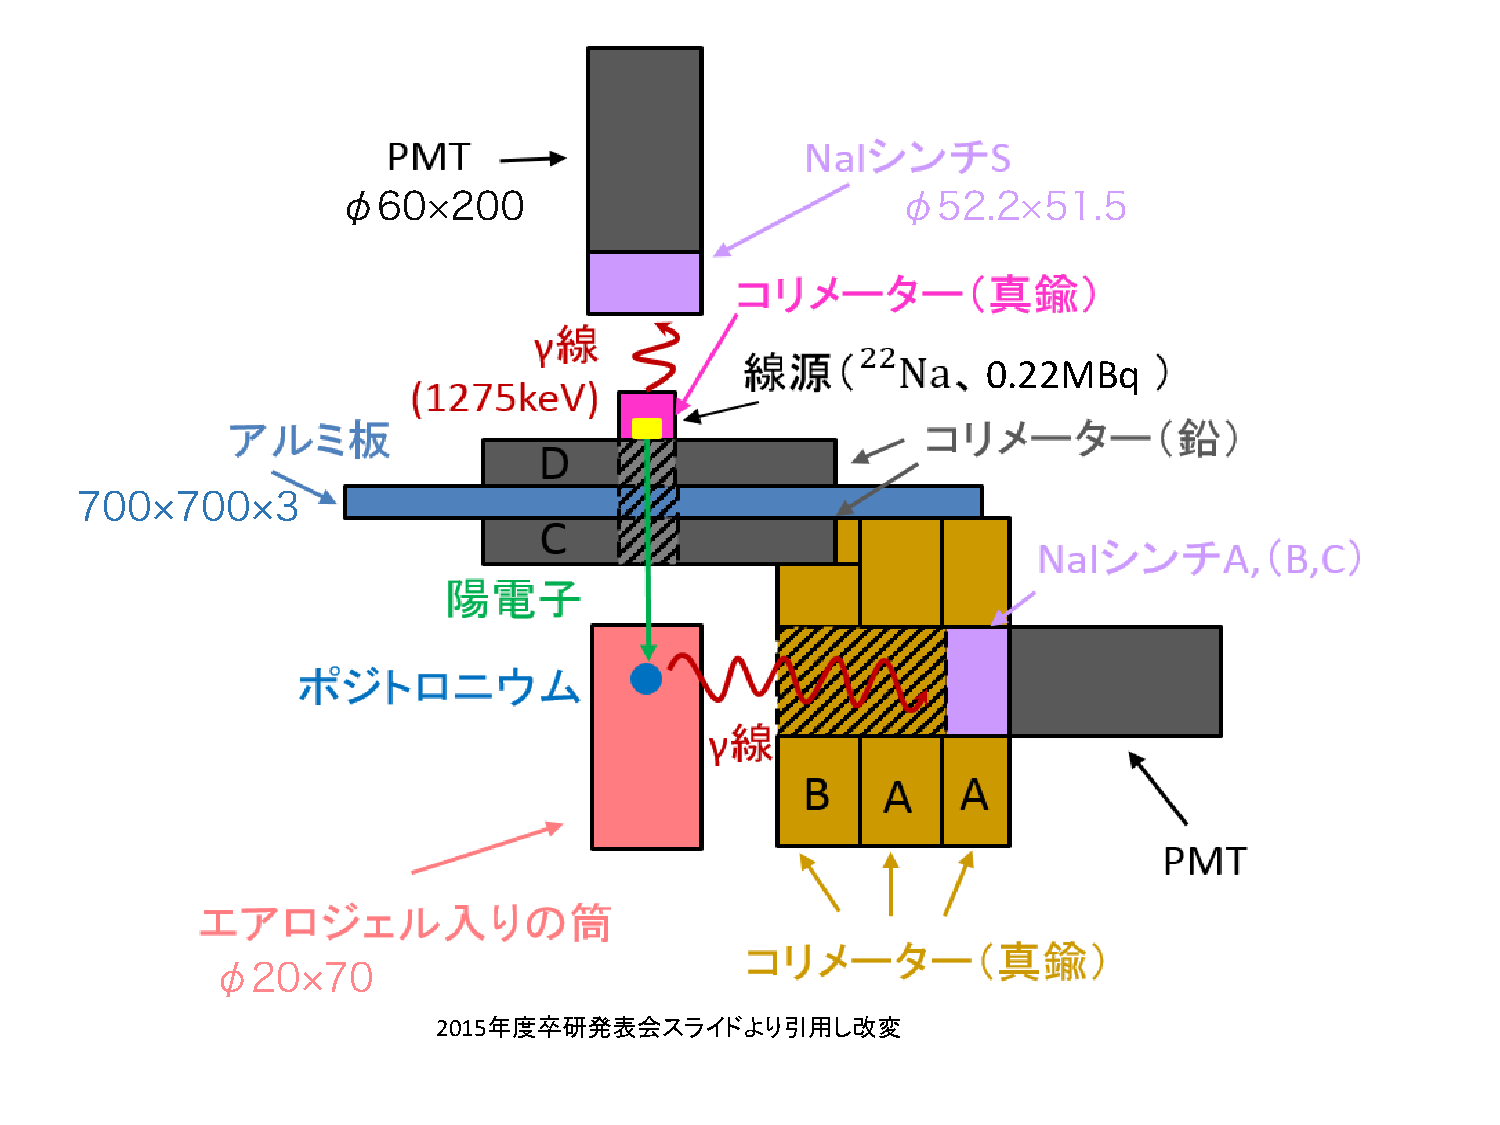
\includegraphics[width=15cm]{fig/isb/settings.pdf}
		\caption{装置の概要図}
		\label{fig:setting_dtl2015}
\end{figure}

イベントは,まず線源に用いている\ce{^{22}Na}からの1275keVのprompt-$\gamma$線を上方に配置されたNaI(Tl)シンチレータSで,下方に陽電子が出てシリカエアロジェル中の電子と反応してポジトロニウムを形成し,崩壊する際に放出する$\gamma$線を下に配置してある3つのNaI(Tl)シンチレータを用いて検出する.
ここで、コリメータをつけているのは線源からの$\gamma$線が直接シンチレータA,B,Cに入射することを防ぐためである.
以下にコリメータの図を昨年度の資料~\cite{卒業発表2015}から引用し示す.

%一気に3行2列で配置する方
%\begin{figure}[H]
%	\begin{minipage}{0.5\hsize}
%		\centering
%		\includegraphics[width=80mm]{fig/isb/collimator1.png}
%		\caption{真鍮製コリメータA}
%		\label{colli1}
%	\end{minipage}
%	\begin{minipage}{0.5\hsize}
%		\centering
%		\includegraphics[width=80mm]{fig/isb/collimator2.png}
%		\caption{真鍮製コリメータB}
%		\label{colli2}
%	\end{minipage}
%	%%%%%%%%%%%%%%%%%%%%%%%%%%%%%%%%%%%%%%%%%%%%%%%%%%%%%%
%	\begin{minipage}{0.5\hsize}
%		\centering
%		\includegraphics[width=80mm]{fig/isb/collimator3.png}
%		\caption{線源用真鍮製コリメータ}
%		\label{colli3_1}
%	\end{minipage}
%	\begin{minipage}{0.5\hsize}
%		\centering
%		\includegraphics[width=80mm]{fig/isb/collimator4.png}
%		\caption{線源用真鍮製コリメータ内部構造}
%		\label{colli3_2}
%	\end{minipage}
%	%%%%%%%%%%%%%%%%%%%%%%%%%%%%%%%%%%%%%%%%%%%%%%%%%%%%%%
%	\begin{minipage}{0.5\hsize}
%		\centering
%		\includegraphics[width=80mm]{fig/isb/leadcollimator2.png}
%		\caption{鉛製コリメータC}
%		\label{leadcolli1}
%	\end{minipage}
%	\begin{minipage}{0.5\hsize}
%		\centering
%		\includegraphics[width=80mm]{fig/isb/leadcollimator1.png}
%		\caption{鉛製コリメータD}
%		\label{leadcolli2}
%	\end{minipage}
%\end{figure}

%1行2列を3つ配置する方
\begin{figure}[H]
	\centering
		\begin{tabular}{c}
			%1枚目
			\begin{minipage}{0.5\hsize}
				\centering
					\includegraphics[width=70mm]{fig/isb/collimator1.png}
					\hspace{1.6cm} (a)真鍮製コリメータ1
			\end{minipage}
			%2枚目
			\begin{minipage}{0.5\hsize}
				\centering
					\includegraphics[width=70mm]{fig/isb/collimator2.png}
					\hspace{1.6cm} (b)真鍮製コリメータ2
			\end{minipage}
		\end{tabular}
\end{figure}
\begin{figure}[H]
	\centering
		\begin{tabular}{c}
			%1枚目
			\begin{minipage}{0.5\hsize}
				\centering
					\includegraphics[width=70mm]{fig/isb/collimator3.png}
					\hspace{1.6cm} (c)真鍮製コリメータ3
			\end{minipage}
			%2枚目
			\begin{minipage}{0.5\hsize}
				\centering
					\includegraphics[width=70mm]{fig/isb/collimator4.png}
					\hspace{1.6cm} (d)真鍮製コリメータ3内部構造
			\end{minipage}
		\end{tabular}
	\end{figure}
\begin{figure}[H]
	\centering
		\begin{tabular}{c}
			%1枚目
			\begin{minipage}{0.5\hsize}
				\centering
					\includegraphics[width=70mm]{fig/isb/leadcollimator1.png}
					\hspace{1.6cm} (e)鉛製コリメータ1
			\end{minipage}
			%2枚目
			\begin{minipage}{0.5\hsize}
				\centering
					\includegraphics[width=70mm]{fig/isb/leadcollimator2.png}
					\hspace{1.6cm} (f)鉛製コリメータ2
			\end{minipage}
		\end{tabular}
		\caption{各コリメータの概要図}
		\label{collimators}
\end{figure}
\newpage
\subsection{回路図}
全体の回路図は図\ref{fig:circuit2015}のようになっており~\cite{卒業論文2015},イベントは次のようにして得られる.
\begin{itemize}
		\item シンチレータSからの信号が2つのdividerを経てdiscriminatorに入り幅800nsのgateを出力する
		\item シンチレータA,B,Cからの信号がSと同様にしてdividerとdiscriminatorを通りOR回路に入る
		\item OR回路を通った後21nsの遅延をかけられ,AND回路に入る.
		\item Sからのgateと同時の信号がやってきた場合にだけ信号が出力されて再度遅延された後ADC gateとTDC stopに到達する.
\end{itemize}
\begin{figure}[htbp]
	\centering
		\includegraphics[width=15cm]{fig/isb/circuit.pdf}
		\caption{再現実験の回路図}
		\label{fig:circuit2015}
\end{figure}

本実験では各シンチレータに入射する$\gamma$線のエネルギーと時刻を測定するためADC,TDCモジュールを用いた.表\ref{module2016}に詳細を示す.
\begin{table}[H]
	\centering
	\begin{tabular}{|c|c|c|r|} \hline
		モジュール & 型番 & シリアルナンバー & 製造会社 \\ \hline \hline
		ADC & V005 & 36211 & 豊伸電子 \\ \hline
		TDC & TMC & KEK 024  & REPIC \\ \hline
	\end{tabular}
	\caption{使用したモジュール}
	\label{module2016}
\end{table}

\subsubsection{discriminatorの閾値}
回路図\ref{fig:circuit2015}に示すようにシンチレータSとシンチレータA,B,Cではそれぞれの回路中にあるdiscriminatorで設定されている閾値が異なる.
\begin{description}
	\item[シンチレータS]\mbox{}\\
		シンチレータSの閾値highは1275keVの$\gamma$線のみを検出するために用いられる.
		highの閾値78.0mVは約900keVのエネルギーに相当する.一方で閾値lowは$\gamma$線の入射時刻を決める役割を持ち,この閾値を下げることで精度を向上させることができる.
		さらにhigh,lowの信号の時間差は事象選別にも利用される.
	\item[シンチレータA,B,C]\mbox{}\\
		シンチレータA,B,CはSよりも低い閾値が設定されている.
		これは閾値highの役割が無関係なノイズを落とすためであり,dividerを通る回数によりhighはlowの2倍の閾値となる.
		lowの役割はSと同様$\gamma$線の入射時刻を決めるものである.
\end{description}

%\subsection{イベントを得る条件}
%イベントは以下のようにして得られる.
%(もう少しわかりやすいように修正するか「実験装置」の節で簡単に述べたのでここはカットする)
%\begin{enumerate}
%	\item シンチレータSに$\gamma$線が入射し2つある閾値を超える
%	\item gate generatorにより幅800nsのcoincidence gateが出力される
%	\item シンチレータA,B,Cのいずれかにオルソポジトロニウムの崩壊由来の$\gamma$線が入り,delayで遅延される
%	\item Sからの信号がAND回路に入って800ns以内にA(B,C)からの信号が来る
%\end{enumerate}

\section{エネルギーの較正}
まず,4つのシンチレータの較正直線を求める.
この再現実験では\ce{^{22}Na}のスペクトルをADCを用いて取得し,2つのピークをそれぞれ既知の511keVと1275keVに対応するものとしてガウス関数でフィットする.
図\ref{fig:calibration_raw_data}較正に用いたデータを示す.
\begin{figure}[H]
	\centering
		\includegraphics[width=11cm]{fig/isb/cal7001.pdf}
		\caption{較正に用いたデータ}
		\label{fig:calibration_raw_data}
\end{figure}
これらのデータに対し図\ref{fig:fit_gauss}のようにガウス関数でフィットし,図\ref{fig:fitA}のような較正直線を得た.
\begin{figure}[htbp]
	\begin{tabular}{cc}
		%1枚目
		\begin{minipage}{0.5\hsize}
			\centering
				\includegraphics[width=80mm]{fig/isb/gaussFit.pdf}
				\caption{ガウス関数によるフィッティング}
				\label{fig:fit_gauss}
		\end{minipage}
		%2枚目
		\begin{minipage}{0.5\hsize}
			\centering
				\includegraphics[width=80mm]{fig/isb/fitA.pdf}
				\caption{Aに対して得られた較正直線}
				\label{fig:fitA}
		\end{minipage}
	\end{tabular}
\end{figure}
\begin{align}
	E_\textrm{A}\textrm{[keV]}=1.79\times {\rm ADC}-174 \nonumber \\ 
	E_\textrm{B}\textrm{[keV]}=1.69\times {\rm ADC}-148 \nonumber \\
	E_\textrm{C}\textrm{[keV]}=1.86\times {\rm ADC}-150 \nonumber \\
	E_\textrm{S}\textrm{[keV]}=1.86\times {\rm ADC}-145 \nonumber
\end{align}
以後,再現実験ではこの較正直線を元にADCとエネルギーの変換を行う.

\section{事象選別の方法と結果}
\subsection{得られたデータ}
本実験で得られたデータを図\ref{fig:dec_t_b4}に示す.
\[
		\left(
			\begin{tabular}{l}
				測定条件:\hspace{8pt}$\textrm{S}\land(\textrm{A}\lor \textrm{B}\lor \textrm{C})$\\
				測定日:2016/12/05  測定時間:27928 sec\\
				run9075  500000 events
			\end{tabular}
		\right)
\]
\begin{figure}[H]
	\centering
		\includegraphics[width=12cm]{fig/isb/decay_t.pdf}
		\caption{崩壊時間の分布}
		\label{fig:dec_t_b4}
\end{figure}

図\ref{fig:dec_t_b4}はシンチレータA,B,Cでの各崩壊時間の分布を足しあげたものである.ここでの崩壊時間はシンチレータSの閾値lowを超えた時刻とシンチレータA,B,Cでの閾値lowを超えた時刻の差である.
t=0付近に見られる鋭いピークは1つのポジトロニウムの崩壊事象由来のものではないアクシデンタルなイベントが多く含まれるために現れるものである.
また,t=800ns付近でイベントが大幅に減少しているのは,シンチレータSの閾値highを超えたときに出力されるcoincidence gateの幅を800nsとしたためである.

\subsection{得られた結果に対する事象選別}
この結果に対し,2種類のカットをかけてバックグラウンド事象を除去しオルソポジトロニウムの崩壊由来の事象を選別する.
\begin{itemize}
	\item low-highカット…光電効果由来1275keVのprompt-$\gamma$線による事象を選別
	\item エネルギーカット…オルソポジトロニウムの崩壊由来の$\gamma$線を選別
\end{itemize}

\subsubsection{シンチレータSに対する事象選別 (low-highカット)}
シンチレータSで観測されるパルスは主に図\ref{fig:pulse_diff}に示すような光電効果によるものとコンプトン散乱によるものの2種類あり,それぞれの特徴としては
\begin{itemize}
	\item 光電効果…波高が大きい
	\item コンプトン散乱…波高が小さい
\end{itemize}
であるがどちらも赤点線で示す立ち上がり時間は一定となる.
\begin{figure}[H]
	\centering
		\includegraphics[width=15cm]{fig/isb/pulse_difference.pdf}
		\caption{パルスの違い}
		\label{fig:pulse_diff}
\end{figure}
このことを利用してシンチレータにエネルギーを落としきらなかったコンプトン散乱事象を排除し,光電効果由来の事象のみを選別する.

図\ref{fig:tHL_all}にシンチレータSに設定された2つの閾値を超えた時間の差,
\begin{center}
	$t_\textrm{HL}=t_\textrm{high}-t_\textrm{low}$
\end{center}
の分布を示す.
\begin{figure}[htbp]
	\begin{tabular}{cc}
		%1枚目
		\begin{minipage}{0.5\hsize}
			\centering
				\includegraphics[width=80mm]{fig/isb/tHL.pdf}
				\caption{$t_\textrm{HL}$の分布}
				\label{fig:tHL_all}
		\end{minipage}
		%2枚目
		\begin{minipage}{0.5\hsize}
			\centering
				\includegraphics[width=80mm]{fig/isb/tHL_cut.pdf}
				\caption{t=30nsまでの$t_\textrm{HL}$分布}
				\label{fig:tHL_zoom}
		\end{minipage}
	\end{tabular}
\end{figure}

$t_\textrm{HL}$=10ns付近に光電効果由来のパルスによるピークが立ち,その後にはコンプトン散乱由来のパルスにより,なだらかなイベント数の減少が確認できる.
図\ref{fig:tHL_zoom}は図\ref{fig:tHL_all}において,$t_\textrm{HL}$=0から30ns付近を拡大したものである.
これより事象選別に利用する$t_\textrm{HL}$の条件として
\begin{center}
	$8\leq$$t_\textrm{HL}$$\leq12$
\end{center}
を採用した.
\subsubsection{シンチレータSに対する事象選別結果}
図\ref{fig:dec_t_cut}にlow-highカット後の崩壊時間分布を示す.
\begin{figure}[H]
	\centering
		\includegraphics[width=10cm]{fig/isb/decay_t_cut.pdf}
		\caption{low-highカット後の崩壊時間分布}
		\label{fig:dec_t_cut}
\end{figure}
low-highカットによりコンプトン散乱由来の事象を含む約76\%のイベントがカットされた.

図\ref{fig:E-tHL}には横軸に信号がシンチレータSの閾値highを超えた時間,縦軸にシンチレータSで観測されたエネルギーを示す.
ここでの時間とはあるoffsetから崩壊時間を引いた値を示している.
%まず,$t_\textrm{high}$が大きくなるに従いエネルギーも大きくなっている特徴的な相関が確認できる.
%このピークの濃い部分は光電効果由来の事象であり,ピークに垂れ下がるように存在する部分はコンプトン散乱由来の事象である.
%また,$t_\textrm{high}=500\sim700$ns付近にもピークが確認できる.
\begin{figure}[H]
	\begin{tabular}{cc}
		%1枚目
		\begin{minipage}{0.5\hsize}
			\centering
				\includegraphics[width=80mm]{fig/isb/E-tHL.pdf}
				\caption{閾値highを超えた時間とエネルギーの関係}
				\label{fig:E-tHL}
		\end{minipage}
		%2枚目
		\begin{minipage}{0.5\hsize}
			\centering
				\includegraphics[width=80mm]{fig/isb/E-tHL_cut.pdf}
				\caption{low-highカット後のhighを超えた時間とエネルギーの関係}
				\label{fig:E-tHL_cut}
		\end{minipage}
	\end{tabular}
\end{figure}
まず,$t_\textrm{high}$が大きくなるに従いエネルギーも大きくなっている特徴的な相関が確認できる.
このピークの濃い部分は光電効果由来の事象であり,ピークに垂れ下がるように存在する部分はコンプトン散乱由来の事象である.
また,$t_\textrm{high}=500\sim700$ns付近にもピークが確認できる.
low-highカットを施したあとの分布を図\ref{fig:E-tHL_cut}に示す.
これより約86\%のイベントがカットされ,$500\sim700$ns付近に存在していたピークを排除することができた.
しかし,比較的エネルギーを大きく落としたコンプトン散乱によるピークは完全に排除できず,残っていることがわかる.

\subsubsection{シンチレータA,B,Cに対する事象選別 (エネルギーカット)}
シンチレータA,B,Cで観測される$\gamma$線のエネルギーは主にポジトロニウムの崩壊由来のもので
\begin{itemize}
		\item $2\gamma$崩壊由来…511keV
		\item $3\gamma$崩壊由来…0$\sim$511keVの連続スペクトル
\end{itemize}
となる.
その他にも線源からの1275keVのprompt-$\gamma$線が直接シンチレータA,B,Cに入ってしまった事象がある.
このカットではポジトロニウムの崩壊由来の$\gamma$線を観測した事象のみを選別する.

前述のようにポジトロニウムの崩壊由来の$\gamma$線は511keVまたは0$\sim$511keVの連続スペクトルとなる.ここでは装置の分解能を考慮に入れて2$\gamma$,3$\gamma$崩壊のエネルギー領域を以下のように定義し,その領域のエネルギーを観測した事象のみを選んだ.
\begin{table}[htbp]
	\centering
		\caption{カットに用いたエネルギー領域}
		\begin{tabular}{|l|c|c|} \hline
			 & $2\gamma$崩壊領域 & $3\gamma$崩壊領域 \\ \hline
			エネルギー & 450$\sim$600 keV & 100$\sim$450 keV\\ \hline
		\end{tabular}
		\label{energy_cut_region}
\end{table}

図\ref{fig:life2gamma}に2$\gamma$領域の,図\ref{fig:life3gamma}に3$\gamma$領域のカットをかける前(青線)とかけた後(赤線)での崩壊時間の分布を示す.
\begin{figure}[htbp]
	\begin{tabular}{cc}
		%1枚目
		\begin{minipage}{0.5\hsize}
			\centering
				\includegraphics[width=80mm]{fig/isb/life_2gamma.pdf}
				\caption{2$\gamma$領域での崩壊時間の分布}
				\label{fig:life2gamma}
		\end{minipage}
		%2枚目
		\begin{minipage}{0.5\hsize}
			\centering
				\includegraphics[width=80mm]{fig/isb/life_3gamma.pdf}
				\caption{3$\gamma$領域での崩壊時間の分布}
				\label{fig:life3gamma}
		\end{minipage}
	\end{tabular}
\end{figure}
カット前後で$2\gamma$領域では80\%が,$3\gamma$領域では34\%の事象が取り除かれたことがわかる.

\section{寿命測定結果}
\subsection{空気中での寿命}
本再現実験ではオルソポジトロニウムの真空中の寿命を直接測定することはできない.
従って,まず空気中での寿命を求めた後昨年度の実験のシミュレーションによって求められた各領域での崩壊比を用いて真空中での寿命を求めることにする.

空気中でのオルソポジトロニウムの寿命は,カットによりバックグラウンドを削減したしたシンチレータA,B,Cの崩壊時間分布のヒストグラムを次の指数関数でフィッティングすることで得られる.
\begin{equation}
	\nonumber
N(t)=N_0\exp(-\frac{t}{\tau_\textrm{air}})+N_\textrm{BG}
\end{equation}
$N_\textrm{BG}$はバックグラウンド事象を考慮したパラメータである.
このフィッティングの結果を図\ref{fig:life_in_air}に示す.
\begin{figure}[H]
	\centering
		\includegraphics[width=10cm]{fig/isb/life_air.pdf}
		\caption{フィッティング結果}
		\label{fig:life_in_air}
\end{figure}
フィッティングの範囲は$(20,500)$であり,800nsを超えたイベントはカットしてある.
このフィットから空気中での寿命$\tau_\textrm{air}$は
\begin{equation}
	\nonumber
	\tau_\textrm{air}=35.7\pm 2.2 \hspace{8pt}(\textrm{ns})
\end{equation}
と測定できた.
この値を用いて真空中でのオルソポジトロニウムの寿命を求めることとした.

\subsection{真空中での寿命}
空気中での寿命$\tau_\textrm{air}=35.7(\textrm{ns})$はスピン交換反応,pick-off反応により真空中での寿命よりも短い寿命が観測される.
今測定したいものは真空中で$3\gamma$崩壊を起こすときのオルソポジトロニウムの寿命である.
これを$\tau_{3\gamma\textrm{vac}}$とすれば,時刻tでまだ崩壊を起こしていないオルソポジトロニウムの個数を$N(t)$とし,$2\gamma$崩壊を起こすオルソポジトロニウムの時定数を$\tau_{2\gamma}$として次の関係式が成り立つ.
\begin{equation}
	-\frac{dN(t)}{dt}=\left(\frac{1}{\tau_{3\gamma\textrm{vac}}}+\frac{1}{\tau_{2\gamma}}\right)N(t)
	\label{eq:2_3gamma}
\end{equation}
今回観測した空気中での寿命$\tau_\textrm{air}$とは
\begin{equation}
	\nonumber
	\frac{1}{\tau_{3\gamma\textrm{vac}}}+\frac{1}{\tau_{2\gamma}}=\frac{1}{\tau_\textrm{air}}
\end{equation}
という関係式が成り立っている.
式\ref{eq:2_3gamma}を変形すると
\begin{equation}
	\nonumber
	-\frac{dN(t)}{dt}=\left(\frac{dN_{3\gamma}}{dt}+\frac{dN_{2\gamma}}{dt}\right)N(t)=\left(\frac{1}{\tau_{3\gamma\textrm{vac}}}+\frac{1}{\tau_{2\gamma}}\right)N(t)
\end{equation}
となり,ここで
\begin{equation}
	\nonumber
	\frac{dN_{3\gamma}}{dN_{2\gamma}}=\frac{\tau_{2\gamma}}{\tau_{3\gamma}}
\end{equation}
よりこれを代入すると
\begin{equation}
	\tau_{3\gamma\textrm{vac}}=\tau_\textrm{air}\left(1+\frac{dN_{2\gamma}}{dN_{3\gamma}}\right)
	\label{eq:life_vacuum}
\end{equation}
となり$\frac{dN_{2\gamma}}{dN_{3\gamma}}$を測定すれば真空中での寿命$\tau_{3\gamma \textrm{vac}}$が求められる.

式\ref{eq:life_vacuum}より崩壊したポジトロニウムのうち,$2\gamma$,$3\gamma$それぞれで崩壊する事象数$N_{2\gamma}$,$N_{3\gamma}$を求めれば真空中での寿命を測定できるが実際には直接的にそれらを求めることはできない.
そのため昨年度の実験~\cite{卒業論文2015}で行ったシミュレーション結果を用いることでこの事象数を決定することとした.
以下にその結果を引用して示す.
\begin{table}[htbp]
	\centering
		\begin{tabular}{|l|c|c|} \hline
			& $2\gamma$崩壊領域 & $3\gamma$崩壊領域 \\ \hline
			$2\gamma$崩壊 & $R_1=19.83\%$ & $R_2=10.15\%$\\
			$3\gamma$崩壊 & $R_3=29.65\%$ & $R_4=0.850\%$\\ \hline
		\end{tabular}
		\caption{崩壊の割合(各事象/観測した事象)}
		\label{2_3gamma_ratio}
\end{table}

$2\gamma$,$3\gamma$崩壊領域で観測される崩壊数を$N_1,N_2$とすると各領域で観測される崩壊数について以下の関係式が成り立つ.
\begin{align}
	N_1=R_1N_{2\gamma}+R_3N_{3\gamma} \\
	N_2=R_2N_{2\gamma}+R_4N_{3\gamma}
	\label{eq:num_of_decay}
\end{align}
式\ref{eq:num_of_decay}より
\begin{align}
	\frac{N_{2\gamma}}{N_{3\gamma}}=\frac{N_1R_4-N_2R_3}{N_2R_1-N_1R_2}
	\label{eq:decay_ratio}
\end{align}
という関係式が得られる.よって式\ref{eq:life_vacuum}と式\ref{eq:decay_ratio}から実験で得られた空気中での寿命を真空中での寿命へ換算できる.

\subsubsection{各エネルギー領域での崩壊数}
実験で観測された崩壊数は$2\gamma$,$3\gamma$崩壊領域の崩壊時間分布のヒストグラムに対し空気中での寿命$\tau_\textrm{air}$を代入した形の式\ref{eq:fit_for_vac}でフィットすることにより得られる.
\begin{align}
	N_0\exp\left(\frac{t}{\tau_\textrm{air}}\right)+N_\textrm{BG} \nonumber \\
	=N_0\exp\left(\frac{t}{35.7}\right)+N_\textrm{BG} 
	\label{eq:fit_for_vac}
\end{align}

フィッティングした結果を以下に示す.フィットの範囲は$(20,500)$である.
\begin{figure}[H]
	\centering
		\includegraphics[width=12cm]{fig/isb/2-3gamma.pdf}
		\caption{フィッティング結果}
		\label{fig:2_3gamma_fit}
\end{figure}
表によりまとめると
\begin{table}[H]
	\begin{tabular}{cc}
	%1つめ
		\begin{minipage}{0.5\hsize}
			\centering
				\begin{tabular}{|c|c|c|}
					\hline
					fit parameter & value \\ \hline
					$N_0$ & $3050 \pm 20$ \\ \hline
					$N_\textrm{BG} $& $174 \pm 2$ \\ \hline
				\end{tabular}
				\caption{$2\gamma$領域でのフィット結果}
		\end{minipage}
	%2つめ
		\begin{minipage}{0.5\hsize}
			\centering
				\begin{tabular}{|c|c|c|}
					\hline
					fit parameter & value \\ \hline
					$N_0$ & $1060 \pm 420$ \\ \hline
					$N_\textrm{BG}$ & $635 \pm 40$ \\ \hline
				\end{tabular}
				\caption{$3\gamma$領域でのフィット結果}
		\end{minipage}
	\end{tabular}
\end{table}
この結果を用いて式\ref{eq:decay_ratio}より$2\gamma,3\gamma$崩壊比は
\begin{equation}
	\nonumber
	\frac{N_{2\gamma}}{N_{3\gamma}}=1.71 \pm 0.26
\end{equation}
となる.

ゆえに真空中でのオルソポジトロニウムの寿命は
\begin{equation}
	\nonumber
	\tau_{3\gamma\textrm{vac}}=96.7 \pm 11.0\hspace{8pt}(\textrm{ns})
\end{equation}
と求まった.
これは理論値$\tau_\textrm{theory}=142\hspace{8pt}(\textrm{ns})$と比較すると$4.12\sigma$の開きがある.

\section{再現実験の考察}
今回の再現実験でオルソポジトロニウムの寿命が$\tau_{3\gamma\textrm{vac}}=96.7 \pm 11.0\hspace{8pt}(\textrm{ns})$と求められた.
ここで昨年度の結果は$\tau_{3\gamma\textrm{vac}}=128 \pm 10(\textrm{ns})$でありこちらは理論値と$1.4\sigma$で一致する.
これは本実験で第\ref{sec:hogehoge}章(←宮辺章を参照)で試験を行ったトリガー用プラスチックシンチレータを新たに導入することを考慮し,昨年度行った別の事象選別を行っておらずバックグラウンドを同程度まで減らすことができなかったためだと考える.\newline

例としてシンチレータSからの信号に対してシンチレータAの信号が$\Delta t(>0)$だけ遅れた場合を考える.
このときシンチレータSからの信号に対し電荷量を積分するためのADC gateは同じく$\Delta t$だけ遅れ,信号は正しく積分されずに見かけ上1275keVよりも小さい電荷量となる.
また,閾値highを超える時間も$\Delta t$だけ小さくなる.%(図を入れるか考え中)%
これは図\ref{fig:E-tHL}と図\ref{fig:E-tHL_cut}ではっきりと確認できていることがわかる.

昨年度はこれを検証するため故意にADC gateを20nsずつずらし相関を調べ,閾値highを超えた時間を10ns毎に分ける作業をlow-highカット後に行っていた.
その後でエネルギー分布からピークと標準偏差を求め$\pm 1\sigma$に含まれるイベントのみを抽出するというカットを行った.

今年度はプラスチックシンチレータを用いて\ce{^{22}Na}の崩壊で放出される陽電子をトリガーに用いる予定である.
この場合,現在の1275keVの$\gamma$線に対し設けている2種の閾値を設定する必要性がなくなり,トリガーの電荷量を測定しなくても問題はない.
それに加え,確実に陽電子がシンチレータA,B,Cの方向へ突き抜けたという情報が与えられるためバックグラウンドの低減にも繋がる予定である.
